%
%  outline latex source document for AV assignment 1.
%  use pdflatex to format this.
%
\documentclass[10pt,a4paper,oneclumn]{article}
\usepackage{amssymb,amsmath}            % if some maths is needed
\usepackage{graphicx}                   % if any images are to be included
% pick a different font if desired
\usepackage{times}

\title{Advanced Vision Assignment 2 Report}  % AILP: please use this title.
\author{Mindaugas Dabulskis, Marat Subkhankulov}                      % replace with name or exam number
\date{26th February 2013}                 % replace with actual date

\begin{document}

\maketitle  % insert title, author info
%
\section{Introduction}

This report describes the work carried out for the second assignment of the AV course.
The aim of the assignment was to track three coloured balls through a set of video frames.
The algorithm for ball detection and segmentation is discussed. 
The performance of the approach is evaluated using a gold standard.

\section{Algorithm and implementation}

In order to detect and track the balls we used the following algorithm:

\begin{enumerate}
\item Apply mask 1 - Average background subtraction
\item Apply mask 2 - Clothing mask based on intensity
\item apply mask 3 - Hand skin mask based on saturation
\item For each ball classify ball pixels based on a training sample
\item Clean up and track the centroids - store the centroid in a matrix
\end{enumerate}

\begin{figure}[h!]
\centering
  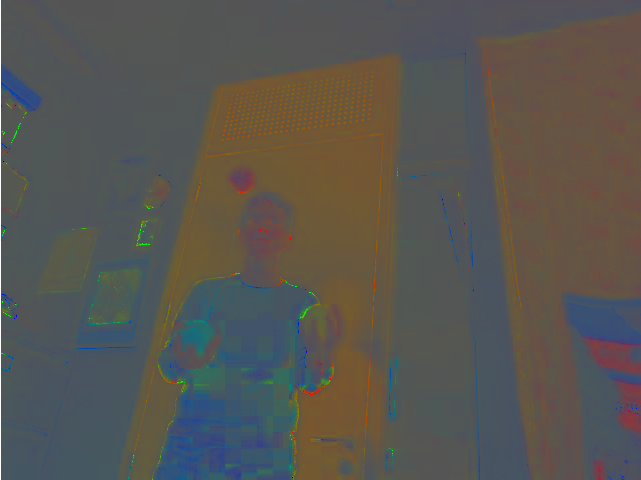
\includegraphics[width=5cm]{figures/imnrgb.png}
  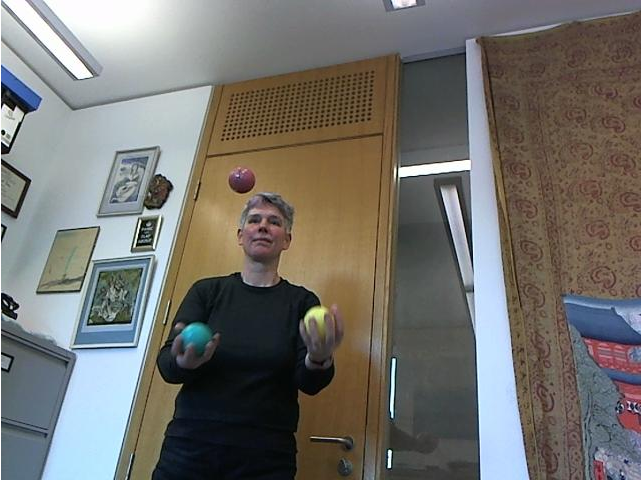
\includegraphics[width=5cm]{figures/original.png}
\caption{Training sample for each ball}
\end{figure}

\subsection{Mask 1: Average background subtraction}

A picture of the empty room had been given, however when subtraction of the background from the subject image did not eliminate the shadow of the door, which had similar values to the yellow ball even in normalized RGB. Thus we obtained a mean of all the frames and used the resulting image as the background; By converting the subject and the new background images to N-RGB, subtracting and thresholding out the low brightness regions we obtained a mask which eliminated the static background, the juggler's, the juggler's face.

\begin{figure}[h!]
\centering
  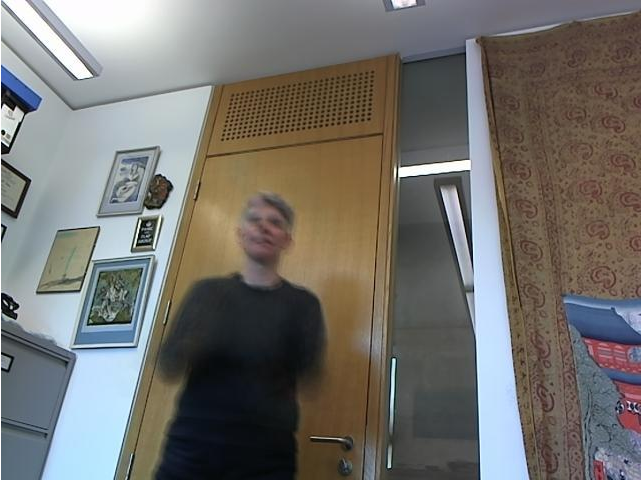
\includegraphics[width=3cm]{figures/av.png}
  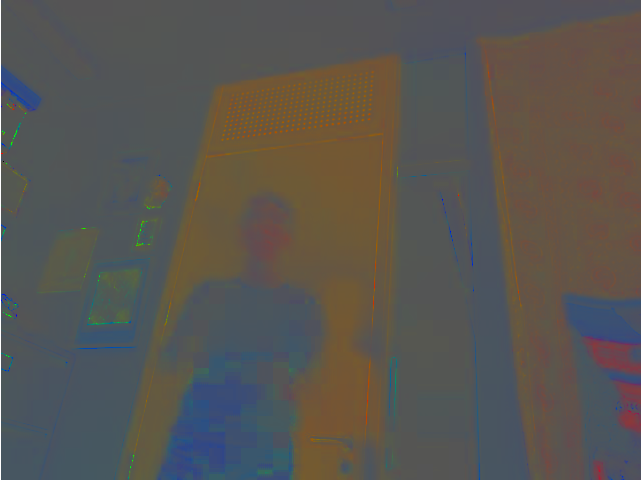
\includegraphics[width=3cm]{figures/avnrgb.png}
  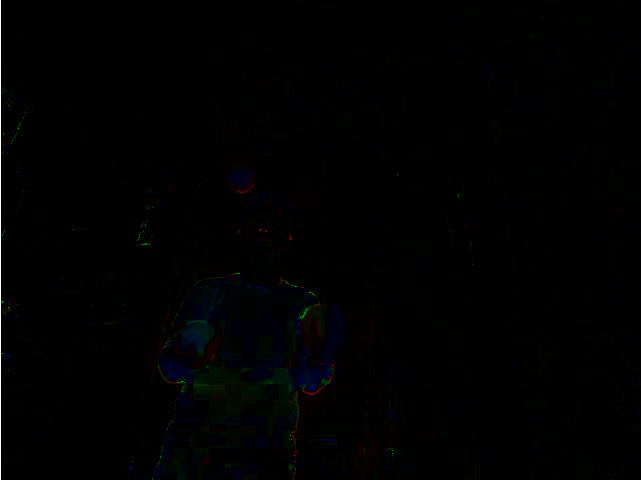
\includegraphics[width=3cm]{figures/avnrgbdif.png}
  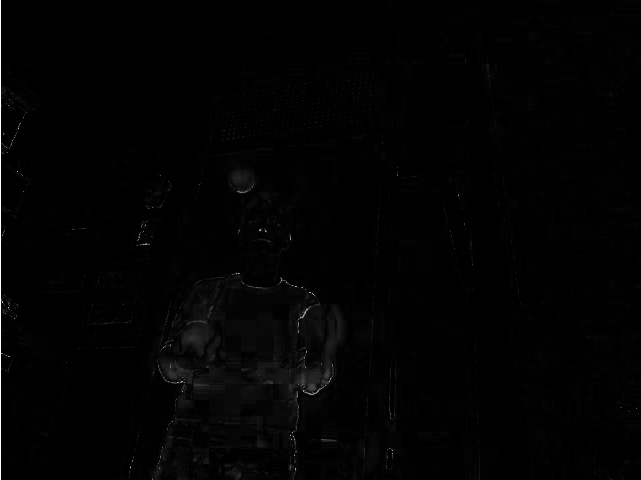
\includegraphics[width=3cm]{figures/avnrgbhsvvalue.png}
  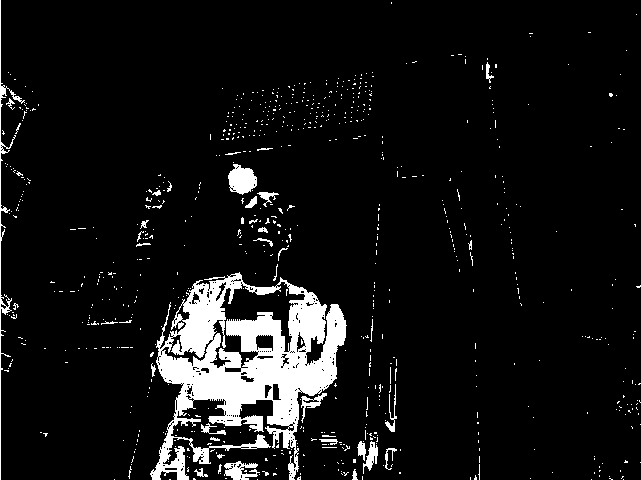
\includegraphics[width=3cm]{figures/avnrgbdifhsvmask.png}
\caption{Training sample for each ball}
\end{figure}

\subsection{Mask 2: Clothing mask}

Mask 1 did not remove the clothing of the juggler due to the smoothing effect of averaging; This posed a problem as the clothes had similar chromaticity to the green ball. We took advantage of the clothes' dark colour to easily theshold out the clothing using a manually set intensity threshold.

\begin{figure}[h!]
\centering
  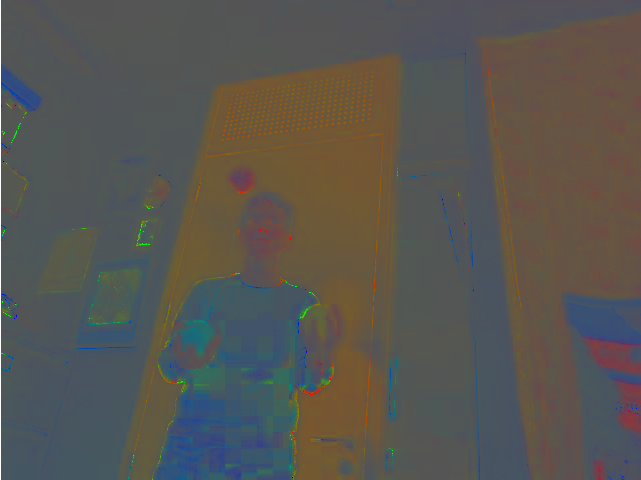
\includegraphics[width=3cm]{figures/imnrgb.png}
  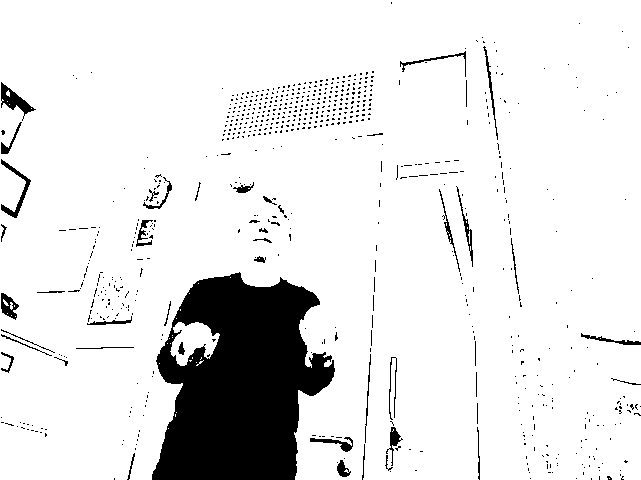
\includegraphics[width=3cm]{figures/clothes_mask.png}
\caption{Training sample for each ball}
\end{figure}

\subsection{Mask 3: Hands}
It seemed reasonable to use N-RGB for segmenting out the balls as the lighting effects were lare largely removed, however the hands of the juggler were not removed by the previous masks and had similar chromaticity to the red ball.The hands were masked by taking advantage of the skin's unique saturation value.

\begin{figure}[h!]
\centering
  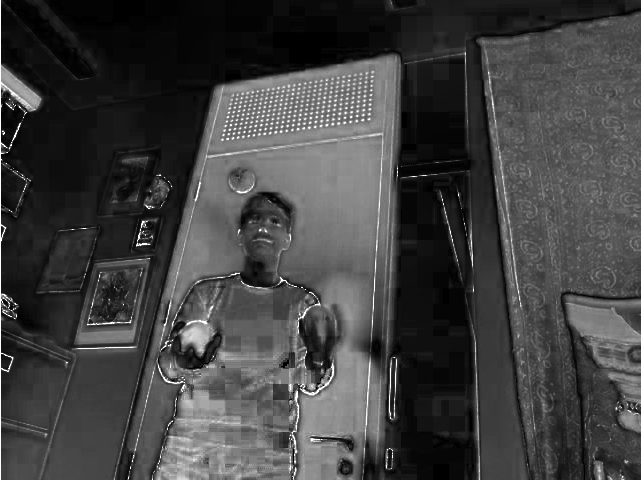
\includegraphics[width=5cm]{figures/imsat.png}
  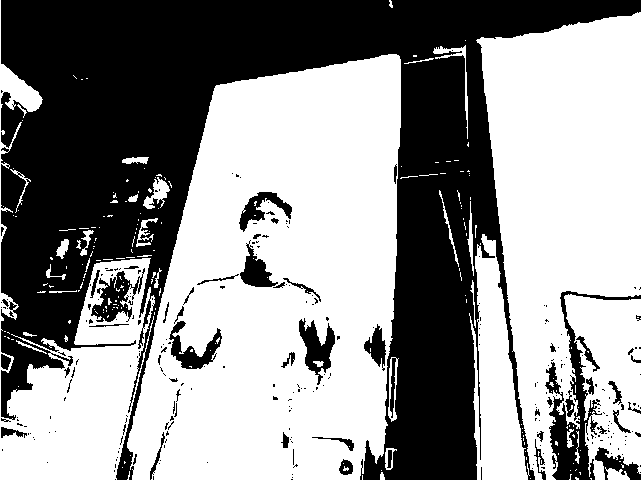
\includegraphics[width=5cm]{figures/imhsvsatmask.png}
\caption{Training sample for each ball}
\end{figure}

\subsection{Classification of ball pixels}

Having applied all of the masks - the background was largely removed. Classification could now be performed. Conversion to N-RGB eliminated diffuse and specular lighting effects on the balls, but necessitated thresholding on all three channels; Since the intensity of all the pixels was largely the same in N-RGB, it was clear that the majority of variation lies in the hue channel - using this single value simplified thresholding as only one channel could be used to successfully classify the ball pixels. 

\begin{figure}[h!]
\centering
  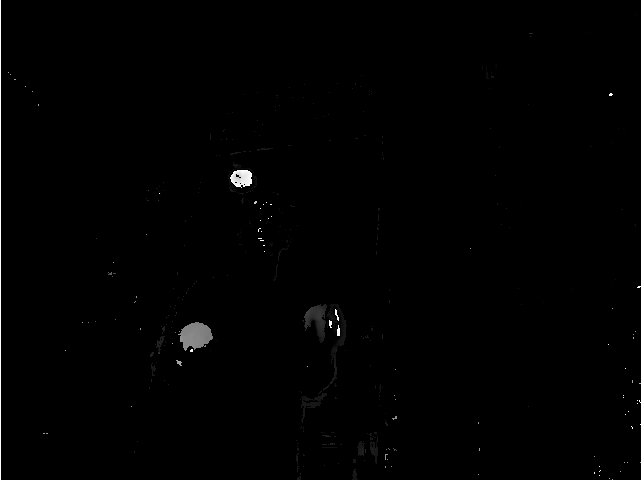
\includegraphics[width=5cm]{figures/bgremoved.png}
\caption{Training sample for each ball}
\end{figure}

Threshold values for hue were obtained from a training sample. The training sample obtained by sampling the pixel at the centroid of each ball given by the ground truth. The lower and upper thresholds were taken at two standard deviations from the median of the sample - this was done to ignore outliers in the sample.

\begin{figure}[h!]
\centering
  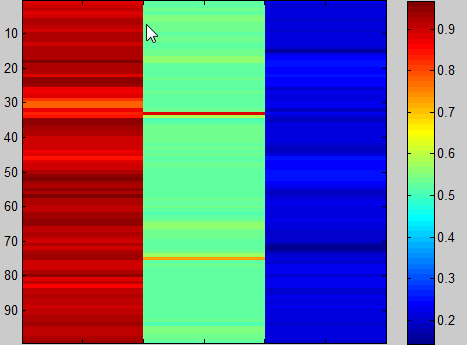
\includegraphics[width=5cm]{figures/training.png}
  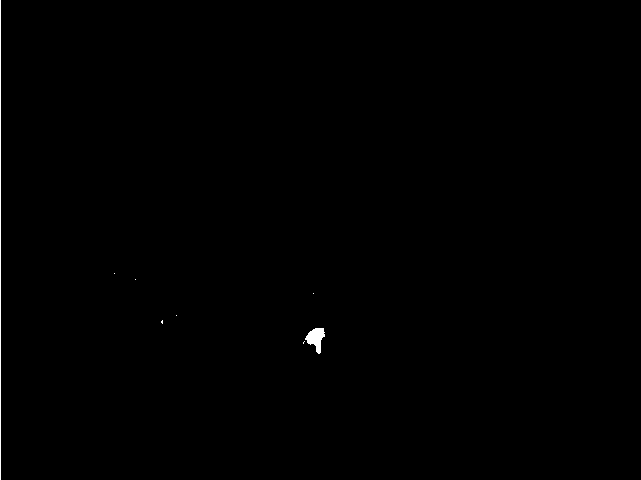
\includegraphics[width=5cm]{figures/class1.png}
  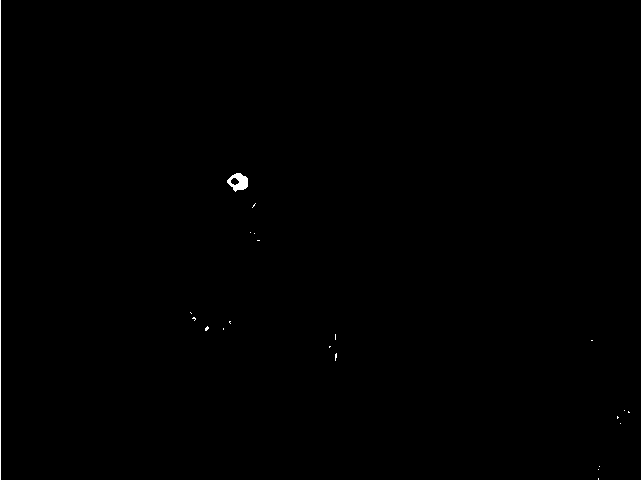
\includegraphics[width=5cm]{figures/class2.png}
  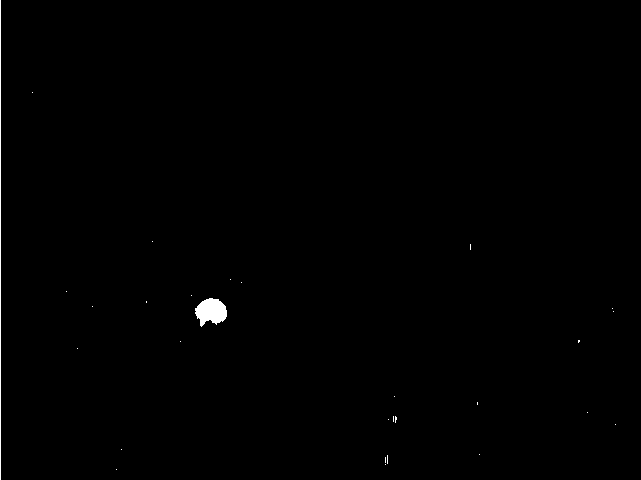
\includegraphics[width=5cm]{figures/class3.png}
\caption{Training sample for each ball}
\end{figure}

\subsection{Clean up and tracking the centroids}

\begin{figure}[h!]
\centering
  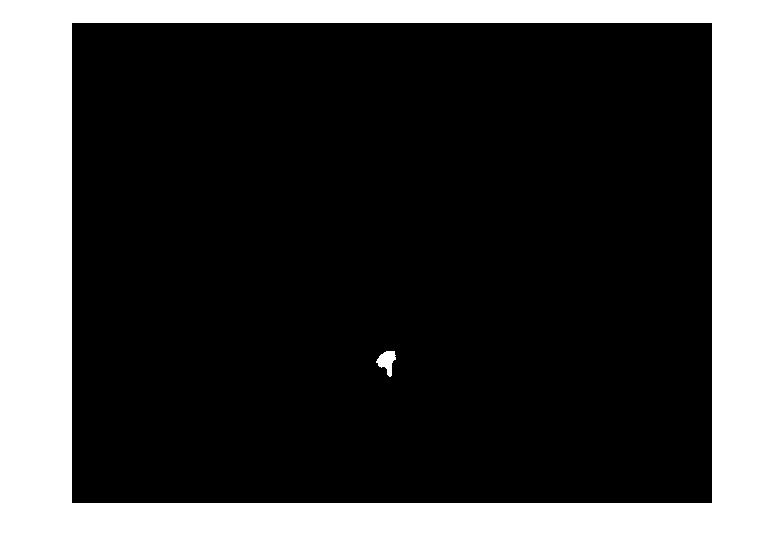
\includegraphics[width=5cm]{cleanedYell.jpg}
  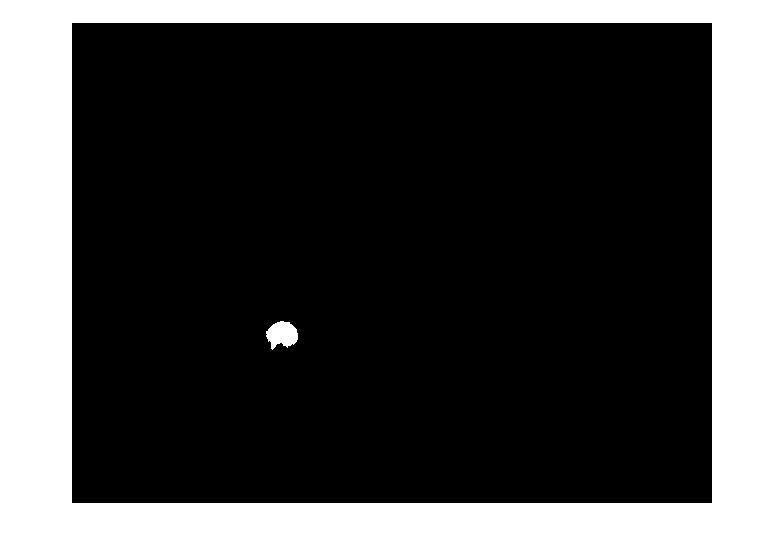
\includegraphics[width=5cm]{cleanGreen.jpg}
  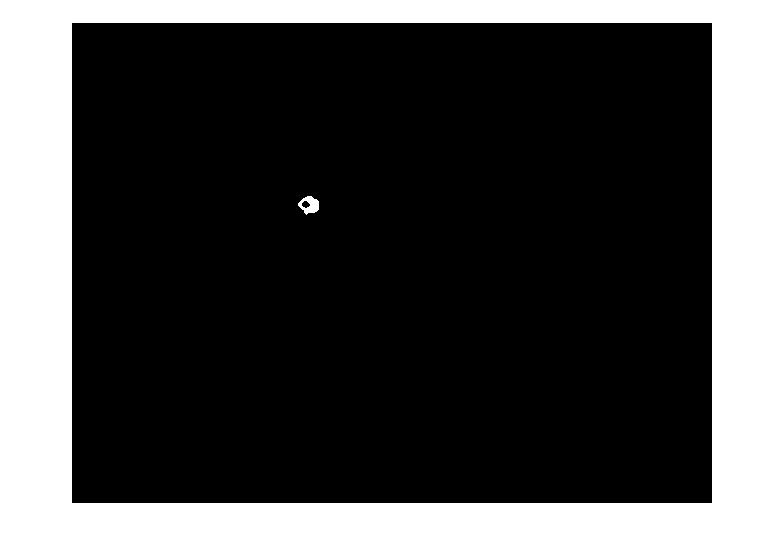
\includegraphics[width=5cm]{cleanRed.jpg}
  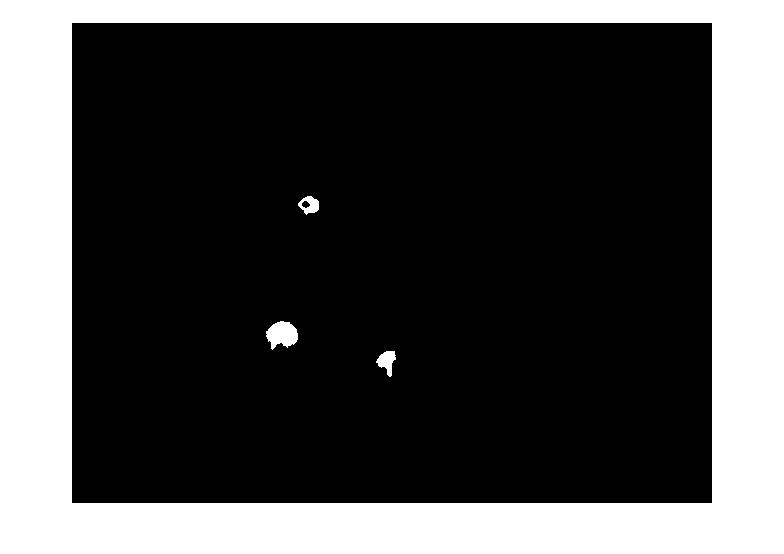
\includegraphics[width=5cm]{cleanAll.jpg}
\caption{Cleaned images}
\end{figure}

Final clean up and ball identification was made using matlab \textbf{bwlabel} and \textbf{regionprops} functions. The function \textbf{bwlabel} takes our intermediate file, which we got after applying all the masks, and labels all the connected objects in the file. Next, this file is supplied to \textbf{regionprops} function, which measures and returns set of the properties for each connected object in the file. Three properties we used:

\begin{enumerate}
\item \emph{Area} - number of actual pixels in the region,
\item \emph{PixelIdxList} - vector containing the linear indices of the pixels in region,
\item \emph{PixelList} - matrix specifying the locations of pixels in the region.
\end{enumerate}

The idea was: 
\begin{enumerate}
\item To find maximum connected object in the file by the pixels area, 
\item Set all other connected object areas pixel to 0 (delete these areas), 
\item Find the middle point of the largest connected objects area. 
\end{enumerate}

Second point cleaned the image of all the noise, because the object with biggest area was the ball itself. Third point was needed for evaluation, to evaluate how much our detected ball differs from ground truth.

\section{Experimental results}

In order to evaluate the algorithm, Euclidean distance between the centroids calculated by the algorithm and the ground truth was measured; A theshold of 10px was set to discriminate between successful and failed detections. In order to qualitatively assess the performance of the algorithm and screen for any outliers the ball trajectories were rendered. In addition we also wanted to find the most appropriate method for calculating the centroid of the detected balls. 
There were three  approaches to calculating the centeroid of the ball, therefore three result sets are presented. These were:

\begin{enumerate}
\item Mean of the area pixels,
\item Median of the area pixels,
\item Maximum and minimum pixels in \textbf{y} and \textbf{x} coordinates and find the mean between them. This creates a bounding box of the area and finds it centre.
\end{enumerate}

\begin{figure}[h!]
\centering
  
\includegraphics{errorCroped.jpg}
\caption{Image in which the distance between ground truth (+) and found mass centre (.) is bigger than 10 pixels}
\end{figure}

\begin{figure}[h!]
\centering
  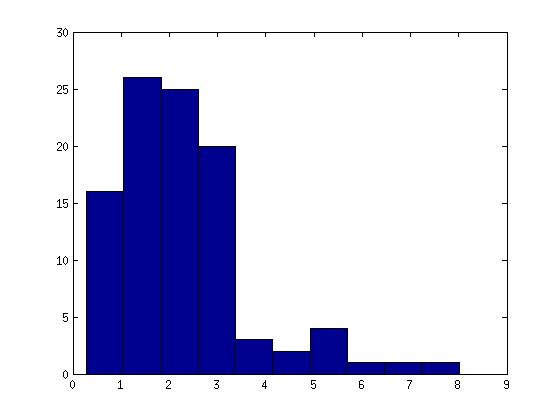
\includegraphics[width=3cm]{redHist.jpg}
  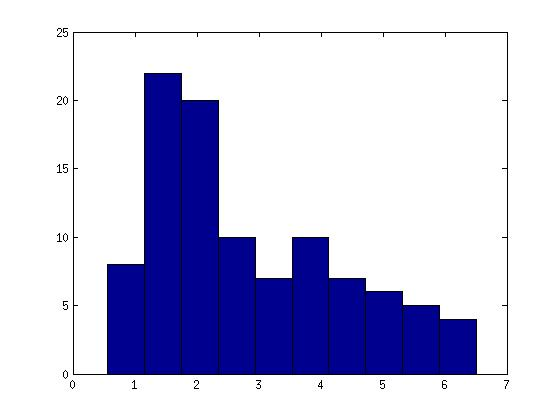
\includegraphics[width=3cm]{greenHist.jpg}
  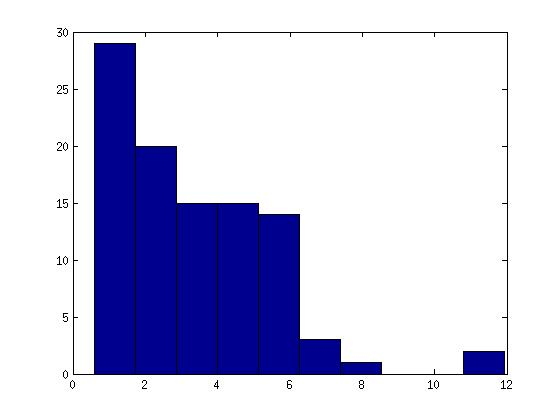
\includegraphics[width=3cm]{yellowHist.jpg}
\caption{Cleaned images}
\end{figure}

\begin{figure}[h!]
\centering
  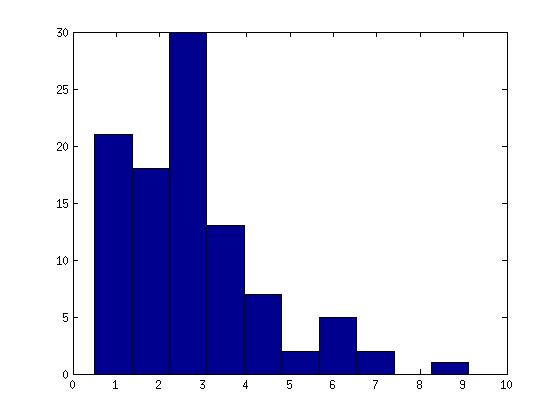
\includegraphics[width=3cm]{redHistBound.jpg}
  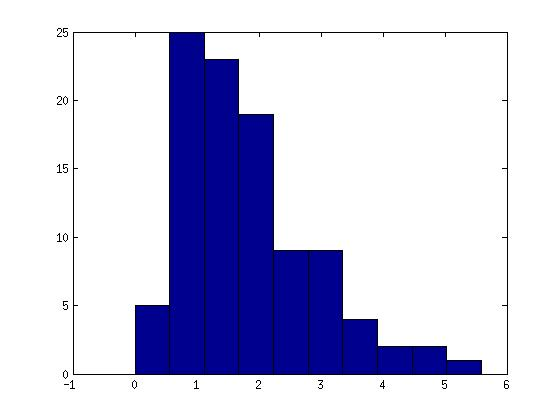
\includegraphics[width=3cm]{greenHistBound.jpg}
  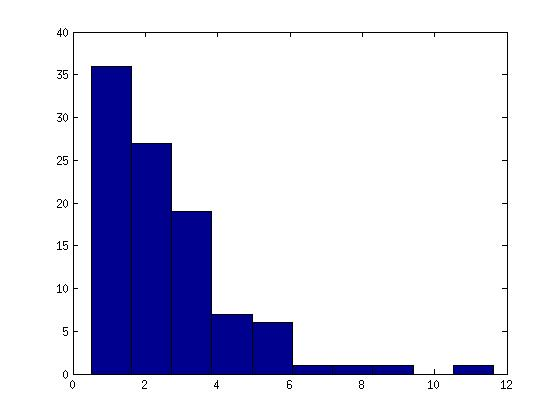
\includegraphics[width=3cm]{yellowHistBound.jpg}
\caption{Cleaned images}
\end{figure}

\begin{figure}[h!]
\centering
  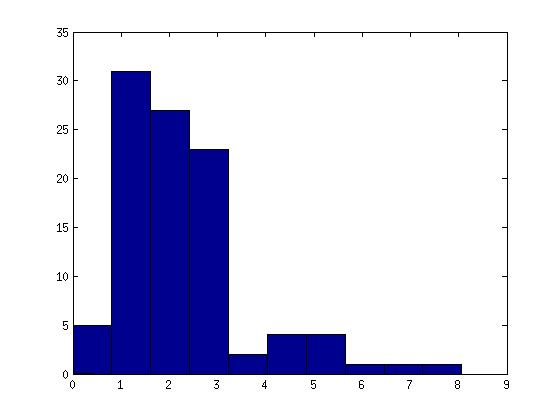
\includegraphics[width=3cm]{redHistMedian.jpg}
  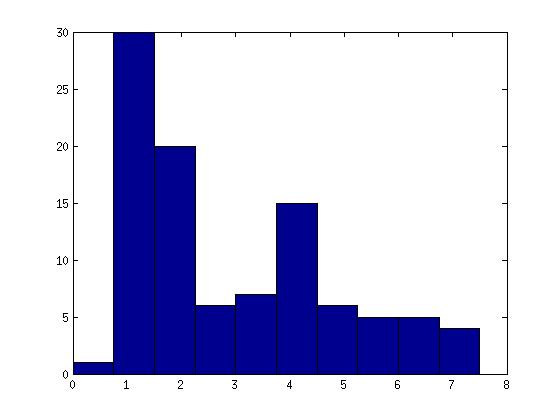
\includegraphics[width=3cm]{greenHistMedian.jpg}
  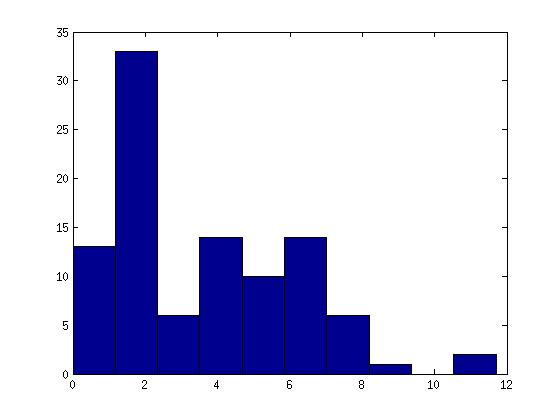
\includegraphics[width=3cm]{yellowHistMedian.jpg}
\caption{Cleaned images}
\end{figure}

\begin{figure}[h!]
\centering
  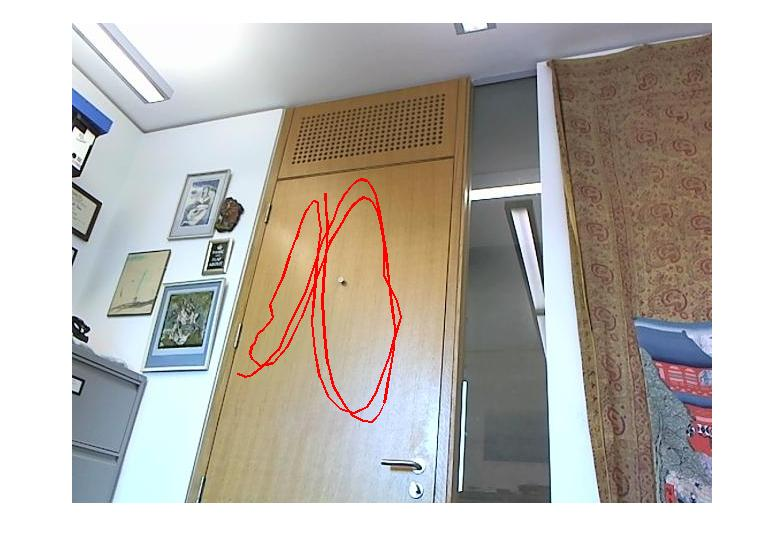
\includegraphics[width=3cm]{redMean.jpg}
  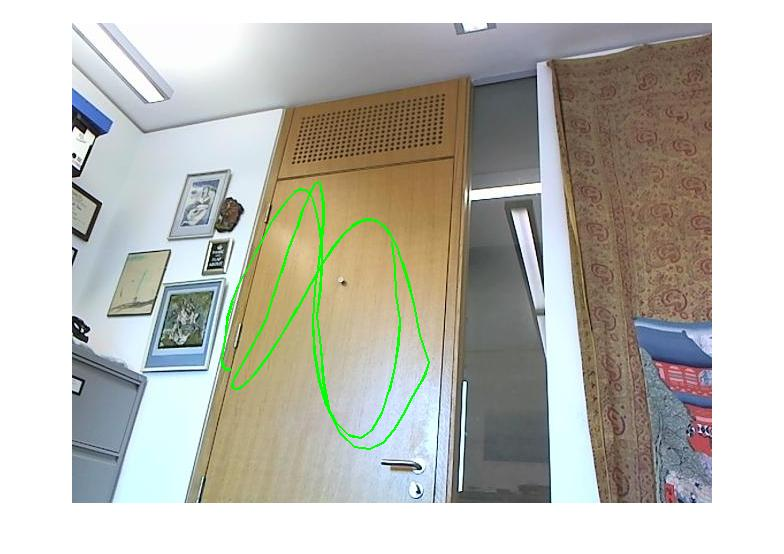
\includegraphics[width=3cm]{greenMean.jpg}
  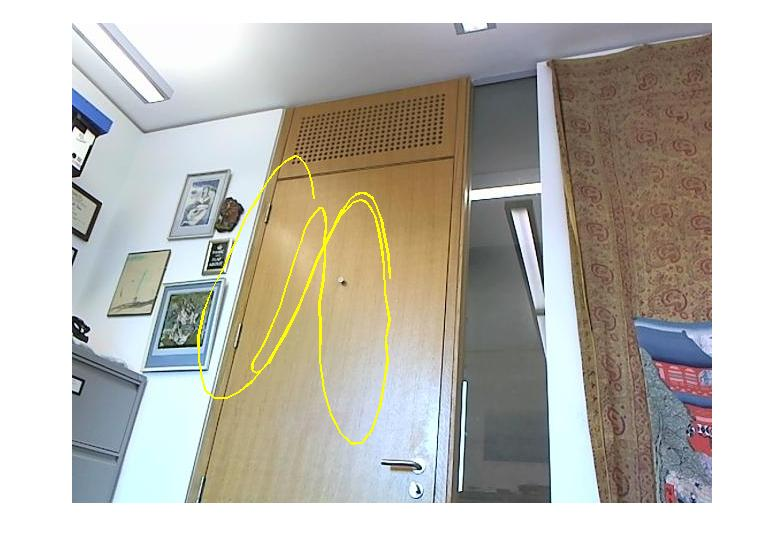
\includegraphics[width=3cm]{yellowMean.jpg}
\caption{Cleaned images}
\end{figure}

\begin{figure}[h!]
\centering
  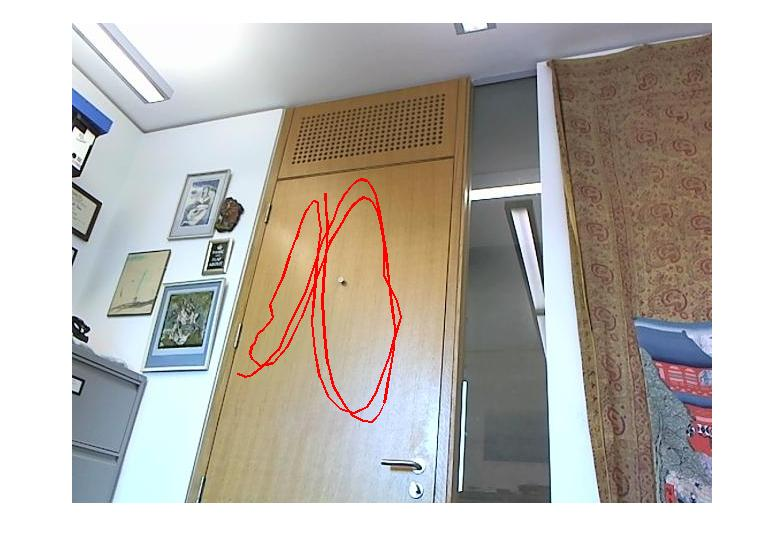
\includegraphics[width=3cm]{redMean.jpg}
  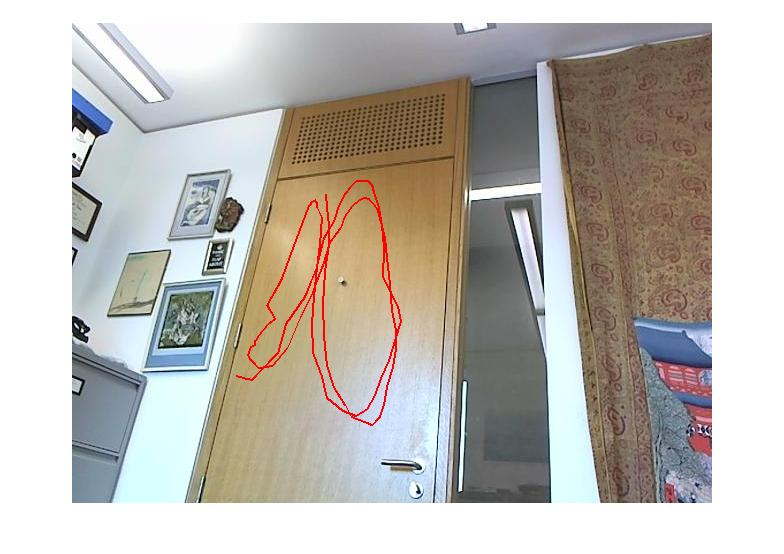
\includegraphics[width=3cm]{redBound.jpg}
  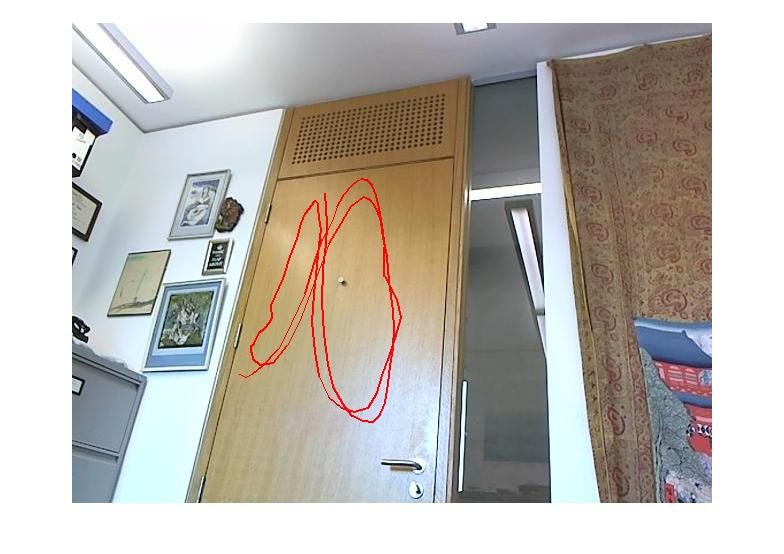
\includegraphics[width=3cm]{medianRedTrack.jpg}
\caption{Cleaned images}
\end{figure}

\begin{table} [h!]
\caption{\label{table1} \textit{Mean}}
\vspace{2mm}
\centerline{
\begin{tabular}{|c|c|c|c|}
\hline
 & Red & Green & Yellow \\
\hline  \hline
ball found in images & 98/98 & 98/98 & 98/98 \\
\hline
mass centre is less than 10 pixels from ground truth & 98/98 & 98/98 & 96/98 \\
\hline
maximum error & 8.0093 &6.5060 &  11.9423 \\
\hline
minimum error & 0.2799 &  0.5622 &  0.5995 \\ 
\hline
one ball error & 224.0428 &   276.9718 & 328.6480 \\
\hline
total error & \multicolumn{3}{|c|}{829.6625} \\
\hline
\end{tabular}}
\end{table}

\begin{table} [h!]
\caption{\label{table1} \textit{Bound}}
\vspace{2mm}
\centerline{
\begin{tabular}{|c|c|c|c|}
\hline
 & Red & Green & Yellow \\
\hline  \hline
ball found in images & 98/98 & 98/98 & 98/98 \\
\hline
mass centre is less than 10 pixels from ground truth & 98/98 & 98/98 & 97/98 \\
\hline
maximum error & 9.1241 &  5.5902&  11.6297 \\
\hline
minimum error &0.5000 20 & 0 & 0.5000\\ 
\hline
one ball error & 264.7848 &  189.4427 & 258.1291 \\
\hline
total error & \multicolumn{3}{|c|}{712.3566} \\
\hline
\end{tabular}}
\end{table}

\begin{table} [h!]
\caption{\label{table1} \textit{Median}}
\vspace{2mm}
\centerline{
\begin{tabular}{|c|c|c|c|}
\hline
 & Red & Green & Yellow \\
\hline  \hline
ball found in images & 98/98 & 98/98 & 98/98 \\
\hline
mass centre is less than 10 pixels from ground truth & 98/98 & 98/98 & 96/98 \\
\hline
maximum error & 8.0623 & 7.5000 & 11.7047 \\
\hline
minimum error & 0 & 0 & 0 \\ 
\hline
one ball error & 227.6602 &   298.2528 & 363.9370 \\
\hline
total error & \multicolumn{3}{|c|}{889.8500} \\
\hline
\end{tabular}}
\end{table}

\section{Discussion}
Qualitative assessment showed 100% detection rate on the training data. There were at most 2 cases of failure - where the centroid deviated from the ground truth above the threshold; Occlusion by the jugglers' fingers is the most likely reason; The fingers occlude half the ball, thus the algorithm segments out only the visible half of the ball and shifts the detected centroid from the ground truth. A potential remedy would be to segment the hands and take the centre of the union of the detected ball and the hand when they are in close proximily. Another approach such as Kalman filtering could be used in conjunction with a motion model to deal with occlusions.

From statistics we can see that bounding box approach has the smallest total error and has only one image in which the centre deviates above threshold, compared to other approaches, which have have two such cases. Using the centre of the bounding box performs well in cases where the ball can be seen through the grasping fingers, so the left, right, top and bottom edges are visible and an accurate centre can be found; However approach is highly sensitive to outliers as any random point can offset it enourmously.

If we look into individual ball error, we notice that with bounding box approach red ball has the largest error compared with other approaches. This is probably caused by the similarity of the hands and the red ball, which causes misclassifications. That is why in mean and median approach the red balls error is smallest, as the outliers are largely ignored; Because of this we decided not to use the bounding box approach.

\subsection{References}

References should be numbered in order of appearance, 
for example \cite{ES1}, \cite{ES2}, and \cite{ES3}. 
You \emph{can} use \texttt{bibtex} to prepare references,
or do it by hand if there are very few.

%
\bibliographystyle{IEEEtran}
\begin{thebibliography}{10}
\bibitem[1]{ES1} Smith, J. O. and Abel, J. S., 
``Bark and {ERB} Bilinear Transforms'', 
IEEE Trans. Speech and Audio Proc., 7(6):697--708, 1999.  
\bibitem[2]{ES2} Lee, K.-F., Automatic Speech Recognition: 
The Development of the 
SPHINX SYSTEM, Kluwer Academic Publishers, Boston, 1989.
\bibitem[3]{ES3} Rudnicky, A. I., Polifroni, Thayer, E. H.,
 and Brennan, R. A.  
"Interactive problem solving with speech", J. Acoust. Soc. Amer., 
Vol. 84, 1988, p S213(A).
\end{thebibliography}

\end{document}
